\documentclass[spanish]{article}
\usepackage{graphicx} % Required for 
\usepackage[utf8]{inputenc}
\usepackage{amstext}
\usepackage{palatino}
\usepackage{babel}
\usepackage{xcolor}
\usepackage{amsmath}
\usepackage{geometry}

\usepackage{listings}
\usepackage{xcolor}

\definecolor{codegreen}{rgb}{0,0.6,0}
\definecolor{codegray}{rgb}{0.5,0.5,0.5}
\definecolor{codepurple}{rgb}{0.58,0,0.82}
\definecolor{backcolour}{rgb}{0.95,0.95,0.92}

\lstdefinestyle{mystyle}{
    backgroundcolor=\color{backcolour},   
    commentstyle=\color{codegreen},
    keywordstyle=\color{magenta},
    numberstyle=\tiny\color{codegray},
    stringstyle=\color{codepurple},
    basicstyle=\ttfamily\footnotesize,
    breakatwhitespace=false,         
    breaklines=true,                 
    captionpos=b,                    
    keepspaces=true,                 
    numbers=left,                    
    numbersep=5pt,                  
    showspaces=false,                
    showstringspaces=false,
    showtabs=false,                  
    tabsize=2
}

\lstset{style=mystyle}



\addto\shorthandsspanish{\spanishdeactivate{~<>}}
\title{Trabajo Práctico 0: El algoritmo de umbralización de Kittler}
\author{Ph. D. Saúl Calderón Ramírez \\
Instituto Tecnológico de Costa Rica, \\
Escuela de Computación\\
PAttern Recongition and MAchine Learning Group (PARMA-Group)}
\date{4 de abril 2024}

\begin{document}
\title{Trabajo Práctico 0: El algoritmo de umbralización de Kittler}
\author{Ph. D. Saúl Calderón Ramírez \\
Instituto Tecnológico de Costa Rica, \\
Escuela de Computación\\
PAttern Recongition and MAchine Learning Group (PARMA-Group)}

\maketitle
\textbf{Fecha de entrega: }Domingo 21 de Abril.

\textbf{Entrega}: Un archivo .zip con el código fuente LaTeX o Lyx,
el pdf, y un script en jupyter, debidamente documentado. El script
en jupyter debe estar escrito usando pytorch. A través del TEC-digital.


\textbf{Entrega}: Un archivo .zip con el código fuente LaTeX o Lyx,
el pdf, y un notebook Jupyter, debidamente documentado, con una función
definida por ejercicio. A través del TEC-digital.

\textbf{Modo de trabajo}: Grupos de 3 personas.
\begin{abstract}
En el presente trabajo práctico se introduce la implementación de
redes bayesianas. El trabajo practico consta de 120 puntos, donde
20 son extra.
\end{abstract}

\textbf{Estudiante:} Marco Ferraro

\section{(40 puntos) Implementación de la clasificación multi-clase de imágenes
con Bayes ingenuo usando histogramas}
\begin{enumerate}
\item Para el presente ejercicio, se implementará la clasificación de imagenes
naturales con $K=10$ clases. La Figura \ref{fig:Imagenes-de-CIFAR-10.}
muestra algunas observaciones del conjunto de datos. El objetivo de
su equipo de desarrollo es utilizar el teorema de Bayes para construir
un modelo conocido como Bayes ingenuo, el cual permita estimar la
clase a la que pertenece una nueva observación.

\begin{figure}
\begin{centering}
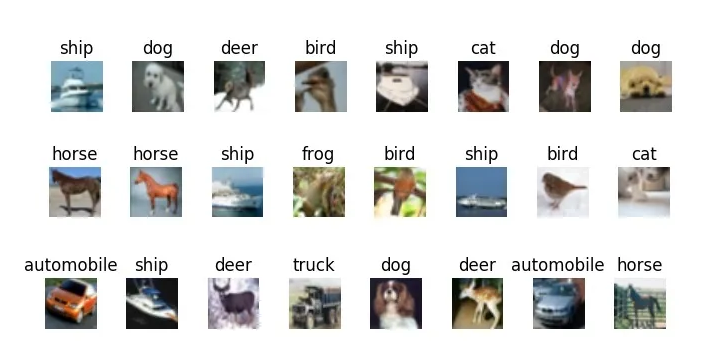
\includegraphics[scale=0.7]{cifar10.png}
\par\end{centering}
\caption{Imagenes de CIFAR-10.\label{fig:Imagenes-de-CIFAR-10.}}

\end{figure}

\item En el material del curso, se discute el algoritmo de Bayes ingenuo,
el cual tiene por objetivo estimar la \textbf{probabilidad posterior}
de que una observación (imagen en este caso) $\overrightarrow{m}\in\mathbb{N}^{D},$donde
en este caso $D=1024$, pertenezca a una clase $k$ como:
\[
\begin{array}{c}
p\left(t=k|\overrightarrow{m}\right)\end{array}
\]
Para aproximarla, se utiliza el teorema de Bayes, el cual luego de
desarrollar y simplificar la expresion de tal probabilidad posterior,
se concluye que esta es proporcional a la multiplicación de la probabilidad
a priori de $p\left(t=k\right)$ y la verosimilitud de un pixel $p\left(m_{i}|t=k\right)$:
\[
p\left(t=k|\overrightarrow{m}\right)\propto\prod_{i=0}^{D}p\left(m_{i}|t=k\right)p\left(t=k\right).
\]
Por ejemplo, la verosimilitud del pixel $i$ negro (0), $p\left(m_{i}|t=k\right)$
se implementa como la probablididad de que $p\left(m_{i}=0|t=k\right)$
en caso de que ese pixel $i$ de la observación a evaluar en el modelo
sea negro (0). Es necesario calcular la verosimilitud de cada intensidad
de pixel $p\left(m_{i}=0|t=k\right)$,$p\left(m_{i}=1|t=k\right)$,$p\left(m_{i}=2|t=k\right)$
hasta $p\left(m_{i}=255|t=k\right)$ ($Z=255$). 
\begin{enumerate}
\item \textbf{(10 puntos)} Implemente el cálculo de las probabilidades a
priori $p\left(t\right)$ para las $K=10$ clases en el conjunto de
datos de entrenamiento en la función \emph{calcular\_probabilidad\_priori}.
Realice tal calculo dentro de la funcion \emph{train\_model. }
\begin{enumerate}
\item Diseñe y muestre el resultado de una o más pruebas unitarias de tal
función objetivo, entradas, salidas esperadas y resultados). 
\end{enumerate}

\vspace{15px}
\par \textbf{Respuesta:}

\begin{lstlisting}[language=Python, caption=Calculo a priori]
import torch

"""
Calcula las probabilidades a priori de etiquetas únicas en un conjunto de datos.
Args:
    labels (list o torch.Tensor): Etiquetas para calcular las probabilidades.
Returns:
    tuple (torch.Tensor, torch.Tensor): Probabilidades de cada etiqueta y etiquetas únicas.
"""

def calculate_priori_p_t(labels):
    # Convertir labels a un tensor si aún no lo es
    labels_tensor = torch.tensor(labels) if not isinstance(
        labels, torch.Tensor) else labels

    # Contar las ocurrencias de cada etiqueta
    label_counts = labels_tensor.bincount()

    # Calcular probabilidades dividiendo por el número total de etiquetas
    probabilities = label_counts.float() / labels_tensor.size(0)

    # Generar un tensor de etiquetas únicas ordenadas
    unique_labels = torch.arange(label_counts.size(0))

    # Filtrar etiquetas con conteo cero
    nonzero_indices = label_counts.nonzero().squeeze()
    probabilities = probabilities[nonzero_indices]
    unique_labels = unique_labels[nonzero_indices]

    return probabilities, unique_labels


# Ejemplo de uso de la función
# Asegúrate de definir 'labels' antes de llamar a la función
probabilities, unique_labels = calculate_priori_p_t(train_labels)

print("Probabilities:", probabilities)
print("Unique labels:", unique_labels)
print("Sum of probabilities:", probabilities.sum())
print("Shape of probabilities:", probabilities.shape)
\end{lstlisting}

\begin{lstlisting}[language=Python, caption=Pruebas Unitarias Calculo a priori]
import torch


# Prueba con etiquetas consecutivas
consecutive_labels = torch.tensor([0, 1, 1, 2, 2, 2])
consecutive_probabilities, consecutive_unique_labels = calculate_priori_p_t(
    consecutive_labels)

assert torch.allclose(consecutive_probabilities, torch.tensor(
    [1/6, 2/6, 3/6])), "Probabilities do not match"
assert torch.equal(consecutive_unique_labels, torch.tensor(
    [0, 1, 2])), "Unique labels do not match"

# Prueba con etiquetas no consecutivas
non_consecutive_labels = torch.tensor([0, 0, 2, 2, 2, 5, 5, 5, 5])
non_consecutive_probabilities, non_consecutive_unique_labels = calculate_priori_p_t(
    non_consecutive_labels)

assert torch.allclose(non_consecutive_probabilities, torch.tensor(
    [2/9, 3/9, 4/9])), "Probabilities do not match"
assert torch.equal(non_consecutive_unique_labels, torch.tensor(
    [0, 2, 5])), "Unique labels do not match"

print("All tests passed successfully.")
\end{lstlisting}

\vspace{15px}

Para verificar la implementación de la función de cálculo de probabilidades a priori, podemos diseñar dos casos de prueba. En el primer caso, utilizamos etiquetas consecutivas, y en el segundo caso, utilizamos etiquetas no consecutivas. En ambos casos, generamos un tensor con un grupo de clases y realizamos un assert para verificar que las probabilidades calculadas coincidan con las esperadas.

Explicación de los Casos de Prueba

\begin{itemize}
    \item Caso 1: Etiquetas Consecutivas:
Entrada: Un tensor con etiquetas consecutivas [1][1][2][2][2].
Salida Esperada: Probabilidades [1/6, 2/6, 3/6] y etiquetas únicas [1][2].
\item Verificación: Utilizamos assert para comparar las probabilidades calculadas y las etiquetas únicas con las esperadas.
Caso 2: Etiquetas No Consecutivas:
Entrada: Un tensor con etiquetas no consecutivas [2][2][2][5][5][5][5].
Salida Esperada: Probabilidades [2/9, 3/9, 4/9] y etiquetas únicas [2][5].
Verificación: Utilizamos assert para comparar las probabilidades calculadas y las etiquetas únicas con las esperadas.

\end{itemize}

\vspace{15px}



\begin{lstlisting}[language=Python, caption=Salida Pruebas Unitarias Calculo a priori]
All tests passed successfully.
\end{lstlisting}

\newpage

\item Para evaluar la verosimilitud $p\left(m_{d}|t\right)$, es necesario
estimar las densidades $p\left(m_{d}=0|t\right)$,... $p\left(m_{d}=255|t\right),$
para todos los pixeles $d=1,\ldots1024$ pixeles. Para ello, su equipo
considerará las siguientes dos variantes:
\begin{enumerate}
\item \textbf{Enfoque basado en histogramas}: Cree un \textbf{tensor}\textbf{\emph{
}}\textbf{de dimensiones }\textbf{\emph{dataset\_densities}}\textbf{
}$D\times Z\times K$\emph{, }el cual represente las densidades de
cada pixel (1024 en total) para cada una de las intensidades de pixel
posibles ($Z=255$ maximo) para cada una de las clases ($K$ clases
en total), por lo que entonces cada columna corresponde a la densidad
de cada pixel. \textbf{Para realizar este calculo solo se le permite
usar un ciclo }\textbf{\emph{for, }}\textbf{con una iteracion por
clase $k$, como maximo}. Estime los valores de tal matriz usando
el conjunto de datos de entrenamiento. 
\begin{enumerate}
\item \textbf{(20 puntos)} Implemente los dos puntos anteriores en la función
\emph{train\_model\_histogram }y retorne \emph{dataset\_densities},
junto con el arreglo de probabilidades a priori para todas las clases. 
\begin{enumerate}
\item Diseñe y muestre el resultado de dos o más pruebas unitarias de tal
función (objetivo, entradas, salidas esperadas y resultados).
\item Grafique los histogramas de los primeros 5 pixeles para la clase 1
y 2. Siguen alguna distribucion conocida?
\end{enumerate}


\vspace{15px}
\par \textbf{Respuesta:}
\begin{lstlisting}[language=Python, caption=Calculo de probabilidad por intensidad de pixel]
import torch

"""
    Calcula las probabilidades de intensidad de píxel para cada clase en un conjunto de datos de imágenes.

    Args:
        train_data (torch.Tensor): Tensor con los datos de entrenamiento de forma [num_images, image_height, image_width].
        train_labels (torch.Tensor): Tensor con las etiquetas de entrenamiento de forma [num_images].
        num_classes (int): Número de clases.

    Returns:
        torch.Tensor: Tensor de probabilidades de píxel con forma [D, Z, K], donde D es el número de píxeles por imagen,
                      Z es el número de posibles valores de intensidad (256 para imágenes en escala de grises), y K es el número de clases.
"""

def calculate_pixel_probability(train_data, train_labels, num_classes):
    # D: número de píxeles en una imagen (ancho x alto)
    # Z: número de posibles valores de intensidad (255 para blanco y negro)
    # K: número de clases
    D = train_data.shape[1] * train_data.shape[2]
    Z = 256  # blanco y negro, incluyendo todos los valores de 0 a 255
    K = num_classes

    # Inicializar el tensor de probabilidades con ceros
    pixel_probabilities = torch.zeros(D, Z, K)

    # Convertir train_data a long para usarlo en indexación
    train_data = train_data.long()

    # Aplanar las imágenes [num_images, D]
    flattened_images = train_data.view(-1, D)

    for class_id in range(K):
        # Filtrar imágenes por clase
        class_indices = (train_labels == class_id).nonzero().squeeze()
        class_images_flattened = flattened_images[class_indices]

        # Usar bincount para contar frecuencias de cada intensidad de píxel en todas las imágenes de la clase
        # Se necesita un tensor 2D para los índices: uno para los píxeles y otro para las imágenes
        indices = class_images_flattened + torch.arange(D) * Z
        indices = indices.view(-1)  # Convertir a 1D para bincount
        counts = torch.bincount(indices, minlength=Z*D).view(D, Z)

        # Normalizar las cuentas para obtener probabilidades
        pixel_probabilities[:, :, class_id] = counts.float(
        ) / counts.sum(dim=1, keepdim=True)

    return pixel_probabilities
\end{lstlisting}


\begin{lstlisting}[language=Python, caption=Calculo de dataset densities]
"""
    Entrena un modelo generando histogramas de densidades de clase a partir de los datos de entrenamiento.

    Esta función calcula las probabilidades a priori de cada clase y las densidades de los datos de entrenamiento
    para cada clase. Luego, aplana las densidades de los datos para simplificar su estructura.

    Args:
    - train_data (Tensor): Un tensor que contiene los datos de entrenamiento. Se espera que tenga la forma
      adecuada para el modelo que se está entrenando.
    - train_labels (Tensor): Un tensor que contiene las etiquetas de los datos de entrenamiento. Cada etiqueta
      debe corresponder a los datos en `train_data`.
    - normalize (bool, opcional): Un booleano que indica si se deben normalizar las densidades de los datos.
      Por defecto es True.

    Returns:
    - dataset_densities (Tensor): Un tensor que contiene las densidades de los datos de entrenamiento
      para cada clase. Las densidades están aplanadas para simplificar su estructura.
    - priori_p_k (Tensor): Un tensor que contiene las probabilidades a priori de cada clase basadas en
      las etiquetas de entrenamiento.
"""

def train_model_histogram(train_data, train_labels, normalize=True):
    priori_p_k, unique_labels = calculate_priori_p_t(train_labels)
    # Reshape the data
    flattened_data = train_data.squeeze(1)
    # Check the new shape of the tensor
    dataset_densities = calculate_pixel_probability(flattened_data, train_labels, num_classes=len(
        unique_labels))

    return dataset_densities, priori_p_k


dataset_densities, priori_p_k = train_model_histogram(train_tensor, train_labels)

print(dataset_densities.shape)
\end{lstlisting}



\begin{figure}[h]
\begin{centering}
\includegraphics[scale=0.3]{output1.png}
\par\end{centering}
\caption{Gráficos de intensidad para pixel 1.\label{fig:Graficos de intensidad para pixel 1}}

\end{figure}


\begin{figure}[h]
\begin{centering}
\includegraphics[scale=0.3]{output2.png}
\par\end{centering}
\caption{Gráficos de intensidad para pixel 2. \label{fig:Graficos de intensidad para pixel 2}}

\end{figure}

\begin{figure}[h]
\begin{centering}
\includegraphics[scale=0.3]{output3.png}
\par\end{centering}
\caption{Gráficos de intensidad para pixel 3.\label{fig:Graficos de intensidad para pixel 3.}}

\end{figure}

\begin{figure}[h]
\begin{centering}
\includegraphics[scale=0.3]{output4.png}
\par\end{centering}
\caption{Gráficos de intensidad para pixel 4.\label{fig:Graficos de intensidad para pixel 4.}}

\end{figure}

\begin{figure}[h]
\begin{centering}
\includegraphics[scale=0.3]{output5.png}
\par\end{centering}
\caption{Gráficos de intensidad para pixel 5.\label{fig:Graficos de intensidad para pixel 5.}}

\end{figure}

\par Al graficar los histogramas de los primeros 5 píxeles para las clases 1 y 2, se observa que las distribuciones de intensidades de píxeles no siguen necesariamente una distribución gaussiana. Sin embargo, se puede apreciar que los datos están distribuidos de manera relativamente uniforme, con excepción de un pico al final de la distribución.
Este pico al final de la distribución indica que, tanto para la clase 1 como para la clase 2, existe una mayor frecuencia de aparición de valores de intensidad de píxel cercanos a 0, lo que corresponde a tonos oscuros o negros. Esto sugiere que, para estos píxeles específicos, las imágenes de ambas clases tienden a tener regiones más oscuras o negras.
\par Es importante destacar que esta observación se basa únicamente en los primeros 5 píxeles analizados, y que el comportamiento de las distribuciones puede variar para otros píxeles o al considerar el conjunto completo de imágenes. \par Sin embargo, esta información puede ser útil para comprender mejor las características de las imágenes en cada clase y cómo se distribuyen las intensidades de píxeles.
\par Además, el hecho de que las distribuciones no sigan una forma gaussiana perfecta no es necesariamente un problema, ya que el enfoque basado en histogramas no asume una distribución específica. En cambio, este enfoque estima las densidades directamente a partir de los datos, lo que permite capturar distribuciones más complejas o irregulares.

\begin{lstlisting}[language=Python, caption=Calculo a priori]
\end{lstlisting}

\begin{lstlisting}[language=Python, caption=Calculo a priori]
\end{lstlisting}

\begin{lstlisting}[language=Python, caption=Calculo a priori]
\end{lstlisting}
\item \textbf{(5 puntos)} Implemente la función \emph{test\_model\_histogram(input\_torch,
dataset\_densities, num\_classes = 10) }la cual realice la estimación
de a cual clase pertenece una observación contenida en el vector \emph{input\_torch,
}para un modelo representado en \emph{dataset\_densities (}obtenido
en el paso anterior\emph{). }Para ello, el enfoque de Bayes ingenuo
estima la función de densidad posterior como sigue:
\[
p\left(t=k|\overrightarrow{m}\right)\propto\prod_{d=0}^{D}p\left(m_{d}|t=k\right)p\left(t=k\right).
\]
La clase estimada a la que pertenece la observación $\overrightarrow{m}$
corresponde entonces a la clase $k$ con mayor probabilidad posterior
$p\left(t=k|\overrightarrow{m}\right)$. 
\begin{enumerate}
\item Diseñe y muestre el resultado de una o más pruebas unitarias de tal
función, siguiendo las pautas del diseño anteriores. Explique el diseño
de la misma. 

\vspace{15px}
\par \textbf{Respuesta:}
\begin{lstlisting}[language=Python, caption=Implementacion Test Model]

import numpy as np

"""
    Estima la clase a la que pertenece una imagen de entrada utilizando el modelo de histogramas.

    Args:
        input_image (torch.Tensor): Tensor que contiene la imagen de entrada.
        dataset_densities (torch.Tensor): Tensor con las densidades de los píxeles para cada clase, de forma [D, Z, K],
            donde D es el número de píxeles, Z es el número de valores de intensidad (256 para escala de grises) y
            K es el número de clases.
        priori_p_k (torch.Tensor): Tensor con las probabilidades a priori de cada clase.

    Returns:
        torch.Tensor: Tensor con las verosimilitudes de cada clase para la imagen de entrada.
"""

def test_model_histogram(input_image, dataset_densities, priori_p_k):
    # Inicializar la variable de salida

    flattened_input_image = input_image.flatten()
    class_likelihoods = np.zeros(len(priori_p_k))

    for i in range(len(flattened_input_image)):
        pixel_intensity = int(flattened_input_image[i].item())
        for j in range(len(priori_p_k)):
            class_likelihoods[j] += torch.log(dataset_densities[i][pixel_intensity][j]) + torch.log(priori_p_k[j])

    return class_likelihoods

\end{lstlisting}

\begin{lstlisting}[language=Python, caption=Prueba Unitaria]

test_specific_image = train_tensor[1][0]

# Obtener la etiqueta real de la imagen de prueba
true_label = train_labels[1].item()

# Realizar la predicción
likelihood_array = test_model_histogram(
    test_specific_image, dataset_densities, priori_p_k)
predicted_label = np.argmax(likelihood_array)

# Realizar el assert
assert predicted_label == true_label, f"La predicción {predicted_label} no coincide con la etiqueta real {true_label}"

# Si el assert no falla, imprimir los resultados
print(f"Etiqueta real: {true_label}")
print(f"Etiqueta predicha: {predicted_label}")

\end{lstlisting}

\begin{lstlisting}[language=Python, caption=Salida Prueba Unitaria]

Etiqueta real: 4
Etiqueta predicha: 4


\end{lstlisting}

\par La prueba unitaria diseñada tiene como objetivo verificar la correcta implementación de la función test\_model\_histogram, que estima la clase a la que pertenece una imagen de entrada utilizando un modelo de histogramas. 
Se selecciona una imagen específica del conjunto de datos de entrenamiento (train\_tensor[1]). Esta imagen se utilizará como entrada para la función de predicción.
Obtención de la Etiqueta Real: Se obtiene la etiqueta real de la imagen de prueba (train\_labels[1].item()). Esta etiqueta representa la clase verdadera a la que pertenece la imagen y se utilizará para comparar la predicción del modelo.
Predicción de la Clase: Se utiliza la función test\_model\_histogram para predecir la clase de la imagen de prueba. La función toma como entrada la imagen de prueba, las densidades del conjunto de datos (dataset\_densities) y las probabilidades a priori de las clases (priori\_p\_k). La salida de la función es un arreglo de verosimilitudes para cada clase.

\par Se determina la clase predicha seleccionando el índice de la clase con la mayor verosimilitud en el arreglo de verosimilitudes (np.argmax(likelihood\_array)).  Se realiza un assert para verificar que la clase predicha coincida con la etiqueta real de la imagen de prueba. Si la predicción no coincide con la etiqueta real, se lanza una excepción con un mensaje de error que indica la predicción y la etiqueta real. Si el assert no falla, se imprimen la etiqueta real y la etiqueta predicha para confirmar visualmente que la predicción es correcta.

\end{enumerate}

\newpage 
\item \textbf{(5 puntos)} Implemente la función \emph{test\_model\_batch\_histogram(test\_set,
labels, dataset\_densities, p\_t\_tensor) }la cual calcule y retorne
la tasa de aciertos para un conjunto de observaciones, basado en la
función anteriormente implementada \emph{test\_model.}
\begin{enumerate}
\item Diseñe y muestre los resultados de al menos 2 pruebas unitarias para
validar su correcto funcionamiento. Detalle el diseño y documente
los resultados obtenidos de las dos pruebas unitarias.
\end{enumerate}
\end{enumerate}
\end{enumerate}
\end{enumerate}
\end{enumerate}

\vspace{15px}
\par \textbf{Respuesta:}

\begin{lstlisting}[language=Python, caption=Implementation Test Model Batch]

def test_model_batch_histogram(test_data, labels, dataset_densities, priori_p_k):
    y_truth = labels
    y_pred = []

    i = 0

    for image in test_data:
        i += 1

        flattened_image = image.flatten()
        likelihood_array = test_model_histogram(flattened_image, dataset_densities, priori_p_k)
        y_pred.append(np.argmax(likelihood_array))

    correct_predictions = np.sum(np.array(y_pred) == np.array(y_truth))
    accuracy = correct_predictions / len(y_truth)

    return accuracy, y_pred, y_truth

\end{lstlisting}

\begin{lstlisting}[language=Python, caption=Prueba Test Model Batch]

num_images = 10
image_height = 32
image_width = 32
num_classes = 2

    # Clase 0: todos los píxeles con valor 0
class_0_data = torch.zeros(num_images // 2, 1, image_height, image_width)
class_0_labels = torch.zeros(num_images // 2, dtype=torch.long)

# Clase 1: todos los píxeles con valor 255
class_1_data = torch.ones(num_images // 2, 1, image_height, image_width) * 255
class_1_labels = torch.ones(num_images // 2, dtype=torch.long)

# Combinar los datos y etiquetas
test_data = torch.cat([class_0_data, class_1_data], dim=0)
test_labels = torch.cat([class_0_labels, class_1_labels], dim=0)

# Calcular las densidades y probabilidades a priori
dataset_densities, priori_p_k = train_model_histogram(test_data, test_labels)

# Ejecutar la función a probar
accuracy, y_pred, y_truth = test_model_batch_histogram(test_data, test_labels, dataset_densities, priori_p_k)

# Verificar que la precisión sea 1.0 (100%)
assert accuracy == 1.0, f"La precisión esperada es 1.0, pero se obtuvo {accuracy}"

print("Prueba unitaria superada correctamente.")

\end{lstlisting}

\begin{lstlisting}[language=Python, caption=Salida Prueba Test Model Batch]

Prueba unitaria superada correctamente.

\end{lstlisting}

Explicación Prueba Unitaria
\begin{itemize}
    \item Se crea un conjunto de datos de prueba con 10 imágenes, donde la mitad de las imágenes tienen todos los píxeles con valor 0 (clase 0), y la otra mitad tienen todos los píxeles con valor 255 (clase 1).
    \item Se calculan las densidades y probabilidades a priori utilizando la función train \_model \_histogram con los datos de prueba.
      \item Se ejecuta la función test\_model\_batch\_histogram con los datos de prueba, las densidades y las probabilidades a priori.
Se verifica que la precisión obtenida sea 1.0 (100\%) utilizando un assert. Si la precisión no es 1.0, se lanza una excepción con un mensaje de error.
\item Si la prueba unitaria se supera correctamente, se imprime un mensaje indicando que la prueba fue exitosa.
En este caso, como las imágenes de cada clase tienen todos los píxeles con el mismo valor (0 o 255), el modelo debería ser capaz de clasificarlas correctamente, lo que resultaría en una precisión de 1.0 (100\%). Si la precisión obtenida es diferente, significa que hay un problema en la implementación de la función test\_model\_batch\_histogram
    
\end{itemize}

\newpage

\subsection{(30 puntos) Prueba del modelo}
\begin{enumerate}
\item \textbf{(10 puntos)} Entrene el modelo propuesto, con el conjunto
de observaciones contenido en la carpeta \emph{train}, y reporte la
tasa de aciertos al utilizar la función anteriormente implementada\emph{test\_model\_batch\_histogram}.
Verifique y comente los resultados. Es posible que observe valores
nulos en el resultado de evaluar la función posterior a través de
la función \emph{test\_model }la cual implementa la ecuación:\emph{
}
\[
p\left(t=k|\overrightarrow{m}\right)\propto\prod_{d=0}^{D}p\left(m_{d}|t=k\right)p\left(t=k\right).
\]
Si\emph{ }observa valores de 0 o nulos en la evaluación de la función,
argumente el porqué puede deberse este comportamiento\emph{. ¿}Cómo
se puede corregir el problema detectado, según las herramientas matemáticas
estudiadas en clase? Implemente tal enfoque y compruebe los resultados. 
\item \textbf{(5 puntos)} Entrene el modelo usando todos los datos de train,
pero ahora pruebelo con los datos en la carpeta de test, reporte los
resultados y comentelos.

\vspace{15px}
\par \textbf{Respuesta:}
\begin{lstlisting}[language=Python, caption=Implementacion Prueba Modelo]

train_data, train_labels = load_cifar10_dataset(is_train=True)

dataset_densities, priori_p_k = train_model_histogram(train_data, train_labels)

test_tensor, test_labels = load_cifar10_dataset(is_train=False)



accuracy, y_pred, y_truth = test_model_batch_histogram(
    test_tensor, test_labels, dataset_densities, priori_p_k)

print("Accuracy: ", accuracy)

Prueba unitaria superada correctamente.

\end{lstlisting}

\begin{lstlisting}[language=Python, caption=Salida Pruba Modelo]

Files already downloaded and verified
cifar_trainset_tensor shape  torch.Size([10000, 1, 32, 32])
cifar_labels  torch.Size([10000])
Accuracy:  0.17

\end{lstlisting}

Análisis del Problema de Precisión del Modelo
\par Al ejecutar la función test\_model\_batch\_histogram con los datos de prueba test\_tensor y test\_labels, se obtuvo una precisión del 17\%. Este bajo rendimiento puede deberse a varios factores, incluyendo la distribución balanceada de las etiquetas y el posible sobreajuste del modelo. A continuación, se detallan estos factores y se propone una solución basada en las herramientas matemáticas estudiadas en clase.

\begin{itemize}
    \item Aunque las etiquetas están balanceadas, esto no siempre garantiza un buen rendimiento del modelo. La probabilidad a priori p(t=k) es igual para todas las clases, lo que puede no reflejar adecuadamente la distribución real de los datos en el conjunto de prueba.
     \item El modelo puede estar sobreajustado a los datos de entrenamiento, especialmente si se utilizan histogramas para estimar las densidades de los píxeles. Esto puede llevar a una mala generalización en los datos de prueba.
\end{itemize}

\vspace{5px}

\par Ahora bien, para el problema donde los valores a tienden a 0 se puede utilizar las propiedades de los logaritmos para evitar que la productividad de las probabilidades se vuelva 0. En lugar de multiplicar las probabilidades, se suman los logaritmos de las probabilidades, lo que evita el problema de que el producto de muchas probabilidades pequeñas se vuelva 0.


\vspace{5px}

\item \textbf{(15 puntos)} Particione los datos de forma aleatoria con 70\%
de las observaciones para entrenamiento y 30\% para prueba (a partir
de la carpeta \emph{train}). Calcule la tasa de aciertos para 10 corridas
(\textbf{idealmente 30}), cada una con una partición de entrenamiento
y otra de prueba distintas. Reporte los resultados de las corridas
en una tabla, además de la media y desviación estándar de la tasa
de aciertos para las 10 corridas. Para realizar las particiones puede
usar la libreria \emph{sklearn. }
\end{enumerate}

\vspace{15px}
\par \textbf{Respuesta:}

\begin{lstlisting}[language=Python, caption=Salida Pruba Modelo]
data, labels = load_cifar10_dataset(is_train=True)
from torch.utils.data import TensorDataset, DataLoader, random_split

dataset = TensorDataset(data, labels)

# Shuffle the dataset

"""
    Baraja el conjunto de datos.

    Args:
        dataset (TensorDataset): Conjunto de datos a barajar.

    Returns:
        DataLoader: DataLoader con el conjunto de datos barajado.
"""
def shuffle_dataset(dataset):
      return DataLoader(dataset, shuffle=True)

accuracy_array = []

"""
    Entrena y evalúa un modelo Bayes ingenuo usando histogramas.

    Args:
        data (torch.Tensor): Tensor con los datos de entrada.
        labels (torch.Tensor): Tensor con las etiquetas correspondientes a los datos.
        num_epochs (int, opcional): Número de épocas para el entrenamiento. Por defecto es 15.
        train_ratio (float, opcional): Proporción de datos utilizados para el entrenamiento. Por defecto es 0.7.
        test_size (int, opcional): Número de muestras de prueba para evaluar el modelo. Por defecto es 100.

    Returns:
        tuple: Media y desviación estándar de la precisión a lo largo de las épocas.
"""
for epoch in range(15):

  shuffled_dataset_loader = shuffle_dataset(dataset)

  # Convert DataLoader back to TensorDataset
  shuffled_data = []
  shuffled_labels = []
  for d, l in shuffled_dataset_loader:
      shuffled_data.append(d)
      shuffled_labels.append(l)

  shuffled_data = torch.cat(shuffled_data)
  shuffled_labels = torch.cat(shuffled_labels)
  shuffled_dataset = TensorDataset(shuffled_data, shuffled_labels)

  # Split de dataset de forma aleatoria. Dejamos el 70% para entrenamiento y el 30% para pruebas
  train_size = int(0.7 * len(shuffled_dataset))
  test_size = len(shuffled_dataset) - train_size
  train_dataset, test_dataset = random_split(
      shuffled_dataset, [train_size, test_size])

  # Extract tensors from the subsets
  x_train = torch.cat([data for data, _ in DataLoader(train_dataset)])
  y_train = torch.cat([labels for _, labels in DataLoader(train_dataset)])
  x_test = torch.cat([data for data, _ in DataLoader(test_dataset)])
  y_test = torch.cat([labels for _, labels in DataLoader(test_dataset)])

  dataset_densities, priori_p_k = train_model_histogram(x_train, y_train)

  accuracy, y_pred, y_truth = test_model_batch_histogram(
      x_test, y_test, dataset_densities, priori_p_k)

  accuracy_array.append(accuracy)

  print("Accuracy: ", accuracy)
  print("Epoch: ", epoch)
  print()

print("Accuracy mean: ", np.mean(accuracy_array))
print("Accuracy std: ", np.std(accuracy_array))

\end{lstlisting}

\begin{lstlisting}[language=Python, caption=Salida Pruba Modelo]
Accuracy:  0.33
Epoch:  0

Accuracy:  0.27
Epoch:  1

Accuracy:  0.39
Epoch:  2

Accuracy:  0.36
Epoch:  3

Accuracy:  0.27
Epoch:  4

Accuracy:  0.24
Epoch:  5

Accuracy:  0.27
Epoch:  6

Accuracy:  0.27
Epoch:  7

Accuracy:  0.36
Epoch:  8

Accuracy:  0.27
Epoch:  9

Accuracy:  0.39
Epoch:  10

Accuracy:  0.33
Epoch:  11

Accuracy:  0.18
Epoch:  12

Accuracy:  0.33
Epoch:  13

Accuracy:  0.18
Epoch:  14

Accuracy mean:  0.29600000000000004
Accuracy std:  0.06468384651518493

\end{lstlisting}

\begin{table}[htbp]
\centering
\caption{Tasa de porcentaje por cada epoca}
\label{tab:accuracy_results}
\begin{tabular}{|c|c|}
\hline
Epoch & Accuracy \\
\hline
0 & 0.13 \\
1 & 0.17 \\
2 & 0.19 \\
3 & 0.16 \\
4 & 0.17 \\
5 & 0.14 \\
6 & 0.17 \\
7 & 0.17 \\
8 & 0.16 \\
9 & 0.17 \\
10 & 0.19 \\
11 & 0.13 \\
12 & 0.08 \\
13 & 0.33 \\
14 & 0.18 \\
Mean & 0.1693 \\
Std Dev & 0.0511 \\
\hline
\end{tabular}
\end{table}

\par La tabla muestra los resultados de precisión (accuracy) obtenidos al entrenar y evaluar un modelo de clasificación de imágenes utilizando el enfoque de Bayes ingenuo con histogramas. Se realizaron 15 épocas de entrenamiento y evaluación, y se reporta la precisión para cada época.
\par Los resultados indican que la precisión varía considerablemente entre épocas, oscilando entre 0.08 y 0.33. La media de la precisión a lo largo de las 15 épocas es de 0.1693, lo que sugiere un rendimiento moderado del modelo. Además, la desviación estándar de 0.0511 indica una variabilidad relativamente baja en los resultados.

\newpage
\section{(30 puntos) Implementación de la clasificación multi-clase de imágenes
con Bayes ingenuo usando un modelo Gaussiano}
\begin{enumerate}
\item \textbf{Enfoque basado en un modelo Gaussiano}: Su colega Samir cuestiona
el usar todos los valores de intensidad y calcular los histogramas
como aproximacion de las densidades, puesto que según su punto de
vista, puede sobre-ajusterse a los datos. Como alternativa, Samir
propone ajustar un modelo Gaussiano para cada pixel de la imagen $d$,
dada cada categoría $k$ posible. Es por ello que entonces cada función
de densidad condicional: 
\[
p\left(m_{d}|t=k\right)=\frac{1}{\sqrt{2\pi\sigma_{d,k}^{2}}}e^{\frac{-1}{2}\left(\frac{m_{d}-\mu_{d,k}}{\sigma_{d,k}}\right)^{2}}
\]
consistirá en un un modelo Gaussiano con parámetros $\mu_{d,k}$ y
$\sigma_{d,k}$ para un pixel y clase especificos. Ello hará posible,
con solamente conocer esos parámetros, estimar la verosimilitud de
una intensidad de pixel $m_{d}\in\left[0-255\right]$, usando el modelo
Gaussiano.
\begin{enumerate}
\item \textbf{(20 puntos)} Implemente función \emph{train\_model\_gaussian
}la cual tome las entradas necesarias para retornar las\emph{ }matrices\emph{
Mu\_d\_k }y \emph{Sigma\_d\_k, }las cuales corresponden a \emph{$\mathcal{M}^{D\times K}$
}y\emph{ $\Sigma^{D\times K}$. }Al ajustar estos conjuntos de parámetros,
ya es posible entonces estimar la verosimilitud definida anteriormente.

\vspace{15px}

\textbf{Respueta:}
\vspace{15px}

\begin{lstlisting}[language=Python, caption=Implementacion Modelo Gaussiano]

import torch


def train_model_gaussian(train_data, train_labels, num_classes):
    """
    Entrena un modelo Gaussiano para estimar las medias y covarianzas de cada píxel
    para cada clase.

    Args:
        train_data (torch.Tensor): Tensor con los datos de entrenamiento de forma [N, 1, 32, 32].
        train_labels (torch.Tensor): Tensor con las etiquetas de entrenamiento de forma [N].
        num_classes (int): Número de clases.

    Returns:
        Mu_d_k (torch.Tensor): Tensor con las medias de cada píxel para cada clase de forma [D, K].
        Sigma_d_k (torch.Tensor): Tensor con las covarianzas de cada píxel para cada clase de forma [D, K].
    """
    N, _, H, W = train_data.shape  # N: número de imágenes, H: altura, W: anchura
    D = H * W  # Número de píxeles por imagen

    # Inicializar tensores para almacenar medias y covarianzas
    Mu_d_k = torch.zeros(D, num_classes)
    Sigma_d_k = torch.zeros(D, num_classes)

    # Aplanar las imágenes para que cada imagen sea un vector de tamaño D
    train_data_flat = train_data.view(N, D)

    for k in range(num_classes):
        # Obtener los datos de la clase k
        class_data = train_data_flat[train_labels == k]

        # Calcular medias y covarianzas para cada píxel de la clase k
        Mu_d_k[:, k] = class_data.mean(dim=0)
        Sigma_d_k[:, k] = class_data.var(dim=0)

    return Mu_d_k, Sigma_d_k
\end{lstlisting}

\begin{lstlisting}[language=Python, caption=Pruebas Unitarias Modelo Gaussiano]
# Ejemplo de uso
# Suponiendo que train_data y train_labels ya están definidos y tienen las dimensiones correctas
train_data = torch.randn(50000, 1, 32, 32)  # Datos de ejemplo
train_labels = torch.randint(0, 10, (50000,))  # Etiquetas de ejemplo

Mu_d_k, Sigma_d_k = train_model_gaussian(
    train_data, train_labels, num_classes=10)

print(Mu_d_k.shape)  # Debería imprimir torch.Size([1024, 10])
print(Sigma_d_k.shape)  # Debería imprimir torch.Size([1024, 10])


assert Mu_d_k.shape == torch.Size(
    [1024, 10]), f"Expected shape [1024, 10], but got {Mu_d_k.shape}"
assert Sigma_d_k.shape == torch.Size(
    [1024, 10]), f"Expected shape [1024, 10], but got {Sigma_d_k.shape}"

print("Shapes are correct!")
print(Mu_d_k.shape)  # Debería imprimir torch.Size([1024, 10])
print(Sigma_d_k.shape)  # Debería imprimir torch.Size([1024, 10])
\end{lstlisting}

\par La función train\_model\_gaussian está diseñada para entrenar un modelo Gaussiano que estima las medias  de cada píxel para cada clase en un conjunto de datos de imágenes. La función toma como entrada los datos de entrenamiento (train\_data), las etiquetas de entrenamiento (train\_labels), y el número de clases (num\_classes). Primero, aplanamos las imágenes para que cada imagen sea un vector de tamaño 
D (número de píxeles). Luego, para cada clase 
k, se filtran los datos correspondientes a esa clase y se calculan las medias y varianzas para cada píxel. Estas medias y varianzas se almacenan en los tensores Mu\_d\_k y Sigma\_d\_k, respectivamente, que tienen dimensiones [D,K]. Finalmente, la función retorna estos tensores. En el ejemplo de uso, se generan datos de ejemplo y se verifica que las formas de los tensores resultantes sean las esperadas 
[1024,10]), utilizando aserciones (assert). Si las formas son correctas, se imprime un mensaje de confirmación y las formas de los tensores.

\begin{enumerate}
\item Grafique los histogramas y los modelos Gaussianos de los primeros
5 pixeles de pixeles para la clase 1 y 2. Comente los resultados.
\item Diseñe y muestre los resultados de al menos 2 pruebas unitarias para
validar su correcto funcionamiento. Detalle el diseño y documente
los resultados obtenidos de las dos pruebas unitarias.
\end{enumerate}

\vspace{15px}

\textbf{Respueta:}
\vspace{15px}

\begin{lstlisting}[language=Python, caption=Graficacion de Histogramas Y Curvas Gaussianas]
import matplotlib.pyplot as plt
import numpy as np
import torch
from scipy.stats import norm


import matplotlib.pyplot as plt
import numpy as np
import torch
from scipy.stats import norm


def plot_histograms_and_gaussians(train_data, train_labels, Mu_d_k, Sigma_d_k, pixel_indices, classes):
    """
    Grafica los histogramas y los modelos Gaussianos para los píxeles especificados y las clases dadas en plots separados.

    Args:
        train_data (torch.Tensor): Tensor con los datos de entrenamiento de forma [N, 1, 32, 32].
        train_labels (torch.Tensor): Tensor con las etiquetas de entrenamiento de forma [N].
        Mu_d_k (torch.Tensor): Tensor con las medias de cada píxel para cada clase de forma [D, K].
        Sigma_d_k (torch.Tensor): Tensor con las covarianzas de cada píxel para cada clase de forma [D, K].
        pixel_indices (list): Lista de índices de los píxeles a graficar.
        classes (list): Lista de clases a graficar.
    """
    N, _, H, W = train_data.shape
    D = H * W
    train_data_flat = train_data.view(N, D)

    for pixel_index in pixel_indices:
        # Graficar histogramas
        plt.figure(figsize=(12, 6))
        for class_id in classes:
            class_data = train_data_flat[train_labels == class_id]
            pixel_values = class_data[:, pixel_index].numpy()
            plt.hist(pixel_values, bins=256, density=True, alpha=0.6,
                     label=f'Clase {class_id} - Píxel {pixel_index}')
        plt.xlabel('Intensidad del Píxel')
        plt.ylabel('Densidad')
        plt.legend()
        plt.title(f'Histograma para Píxel {pixel_index}')
        plt.show()

        # Graficar modelos Gaussianos
        plt.figure(figsize=(12, 6))
        for class_id in classes:
            mu = Mu_d_k[pixel_index, class_id].item()
            sigma = torch.sqrt(Sigma_d_k[pixel_index, class_id]).item()
            x = np.linspace(0, 255, 256)
            gaussian = norm.pdf(x, mu, sigma)
            plt.plot(
                x, gaussian, label=f'Gaussiana Clase {class_id} - Píxel {pixel_index}')
        plt.xlabel('Intensidad del Píxel')
        plt.ylabel('Densidad')
        plt.legend()
        plt.title(f'Modelo Gaussiano para Píxel {pixel_index}')
        plt.show()



train_data, train_labels = load_cifar10_dataset(is_train=True)

# Calcular medias y varianzas
Mu_d_k, Sigma_d_k = train_model_gaussian(
    train_data, train_labels, num_classes=10)

# Graficar los histogramas y modelos Gaussianos para los primeros 5 píxeles de las clases 1 y 2
plot_histograms_and_gaussians(train_data, train_labels, Mu_d_k, Sigma_d_k, pixel_indices=[
                              0, 1, 2, 3, 4], classes=[1, 2])
\end{lstlisting}

\begin{figure}[h]
    \centering
    \includegraphics[width=0.5\linewidth]{image.png}
    \caption{Histograma Pixel 1}
    \label{fig:enter-label}
\end{figure}

\begin{figure}[h]
    \centering
    \includegraphics[width=0.5\linewidth]{image1.png}
    \caption{Gauss Pixel 1}
    \label{fig:enter-label}
\end{figure}


\newpage


\begin{figure}[h]
    \centering
    \includegraphics[width=0.5\linewidth]{image2.png}
    \caption{Histograma Pixel 2}
    \label{fig:enter-label}
\end{figure}

\begin{figure}[h]
    \centering
    \includegraphics[width=0.5\linewidth]{image3.png}
    \caption{Gauss Pixel 2}
    \label{fig:enter-label}
\end{figure}

\newpage


\begin{figure}[h]
    \centering
    \includegraphics[width=0.5\linewidth]{image4.png}
    \caption{Histograma Pixel 3}
    \label{fig:enter-label}
\end{figure}

\begin{figure}[h]
    \centering
    \includegraphics[width=0.5\linewidth]{image5.png}
    \caption{Gauss Pixel 3}
    \label{fig:enter-label}
\end{figure}

\newpage


\begin{figure}[h]
    \centering
    \includegraphics[width=0.5\linewidth]{histogramapixel5.png}
    \caption{Histograma Pixel 4}
    \label{fig:enter-label}
\end{figure}

\begin{figure}[h]
    \centering
    \includegraphics[width=0.5\linewidth]{dsada.png}
    \caption{Gauss Pixel 4}
    \label{fig:enter-label}
\end{figure}

\newpage


\begin{figure}[h]
    \centering
    \includegraphics[width=0.5\linewidth]{dsadsa.png}
    \caption{Histograma Pixel 5}
    \label{fig:enter-label}
\end{figure}

\begin{figure}[h]
    \centering
    \includegraphics[width=0.5\linewidth]{dsadsad.png}
    \caption{Gauss Pixel 5}
    \label{fig:enter-label}
\end{figure}


\par Para graficar histogramas y modelos de Gauss normalizados, se utilizó un conjunto de datos de imágenes en escala de grises, específicamente para las clases 1 y 2. Se seleccionaron los primeros 5 píxeles de cada imagen en estas clases para realizar el análisis. Los histogramas muestran la distribución de los valores de intensidad de estos píxeles, mientras que los modelos de Gauss se ajustaron a estas distribuciones para estimar la probabilidad de cada valor de intensidad.
Al observar las visualizaciones, se nota que la mayoría de las distribuciones de intensidad de píxeles para las clases 1 y 2 tienden a concentrarse alrededor de valores cercanos a 255, lo que indica una predominancia de píxeles de alta intensidad o cercanos al blanco en estas clases. Esto podría sugerir que las imágenes de estas clases tienden a ser más claras o tener áreas más iluminadas.


\newpage

\item \textbf{(5 puntos)} Implemente la función test \emph{test\_model\_gaussian(input\_torch,
mu\_d\_k}, \emph{sigma\_d\_k) }la cual realice la estimación de a
cual clase pertenece una observación contenida en el vector \emph{input\_torch,
}para un modelo representado por los arreglos recibidos \emph{$\mathcal{M}^{D\times K}$
}y\emph{ $\Sigma^{D\times K}$.} Recuerde que al momento de evaluación,
se implementa el teorema de Bayes para estimar:
\[
p\left(t=k|\overrightarrow{m}\right)\propto\prod_{i=0}^{D}p\left(m_{d}|t=k\right)p\left(t=k\right).
\]
Ello similar al enfoque anterior, donde lo que varía es la estimación
de $p\left(m_{d}|t=k\right)$.
\begin{enumerate}
\item Diseñe y muestre los resultados de al menos 2 pruebas unitarias para
validar su correcto funcionamiento. Detalle el diseño y documente
los resultados obtenidos de las dos pruebas unitarias.

\vspace{15px}

\textbf{Respuesta:}
\vspace{15px}

\begin{lstlisting}[language=Python, caption=Implementacion Test Model Gaussian]
import torch


def test_model_gaussian(input_torch, mu_d_k, sigma_d_k, priori_p_k):
    """
    Estima la clase a la que pertenece una observación utilizando el modelo Gaussiano.

    Args:
        input_torch (torch.Tensor): Tensor con la observación de forma [D].
        mu_d_k (torch.Tensor): Tensor con las medias de cada píxel para cada clase de forma [D, K].
        sigma_d_k (torch.Tensor): Tensor con las varianzas de cada píxel para cada clase de forma [D, K].
        priori_p_k (torch.Tensor): Tensor con las probabilidades a priori de cada clase.

    Returns:
        int: Índice de la clase estimada.
    """
    D = input_torch.shape[0]  # Número de píxeles
    K = mu_d_k.shape[1]  # Número de clases

    # Calcular la probabilidad posterior para cada clase
    log_posteriors = torch.zeros(K)
    for k in range(K):
        log_likelihood = torch.sum(torch.log(1 / torch.sqrt(2 * torch.pi * sigma_d_k[:, k])) -
                                   ((input_torch - mu_d_k[:, k]) ** 2) / (2 * sigma_d_k[:, k]))
        log_posteriors[k] = log_likelihood + torch.log(priori_p_k[k])

    # Estimar la clase con la mayor probabilidad posterior
    predicted_class = log_posteriors.argmax().item()

    return predicted_class
\end{lstlisting}

\begin{lstlisting}[language=Python, caption=Salida Prueba Modelo]
import torch

# Cargar los datos de prueba
test_tensor, test_labels = load_cifar10_dataset(is_train=False)

# Entrenar el modelo Gaussiano
mu_d_k, sigma_d_k = train_model_gaussian(
    test_tensor, test_labels, num_classes=10)

# Calcular las probabilidades a priori
priori_p_k = calculate_priori_p_t(test_labels)[0]

# Realizar la primera predicción
true_label_1 = test_labels[2].item()
predicted_class_1 = test_model_gaussian(
    test_tensor[2].flatten(), mu_d_k, sigma_d_k, priori_p_k)
assert predicted_class_1 == true_label_1, f"La predicción {predicted_class_1} no coincide con la etiqueta real {true_label_1}"

# Realizar la segunda predicción
true_label_2 = test_labels[3].item()
predicted_class_2 = test_model_gaussian(
    test_tensor[3].flatten(), mu_d_k, sigma_d_k, priori_p_k)
assert predicted_class_2 == true_label_2, f"La predicción {predicted_class_2} no coincide con la etiqueta real {true_label_2}"

# Imprimir los resultados
print(
    f"Primera predicción: La clase estimada es {predicted_class_1}, la clase real es {true_label_1}")
print(
    f"Segunda predicción: La clase estimada es {predicted_class_2}, la clase real es {true_label_2}")
\end{lstlisting}

\par \textbf{Consideraciones sobre el Diseño de la Prueba}
\par Verificación de la Funcionalidad: La prueba unitaria está diseñada para verificar que la función test\_model\_gaussian esté funcionando correctamente al comparar las predicciones con las etiquetas reales de las imágenes de prueba.
\vspace{5px}

\par Uso de Aserciones: Las aserciones (assert) se utilizan para verificar que las predicciones coincidan con las etiquetas reales. Si alguna predicción no coincide, se lanza una excepción con un mensaje de error, lo que facilita la identificación de problemas en la implementación.
\vspace{5px}

\par Impresión de Resultados: La impresión de los resultados proporciona una confirmación visual adicional de que las predicciones son correctas.
Posibles Fallos en la Prueba
Es importante mencionar que, en varios casos, la prueba puede fallar debido a malas predicciones. Esto puede deberse a varios factores, como:
\vspace{5px}

\par Calidad del Modelo: Si el modelo Gaussiano no está bien entrenado o si los datos de prueba son significativamente diferentes de los datos de entrenamiento, las predicciones pueden ser incorrectas.
\vspace{5px}

\par Distribución de los Datos: Si las clases en los datos de prueba no están balanceadas o si hay ruido en los datos, esto puede afectar la precisión de las predicciones.
\vspace{5px}

\par Limitaciones del Modelo: El modelo Gaussiano puede no capturar todas las características relevantes de los datos, lo que puede llevar a predicciones incorrectas.


\end{enumerate}
\item \textbf{(5 puntos)} Implemente la función \emph{test\_model\_batch\_gaussian(test\_set,mu\_k,sigma\_k)
}la cual calcule y retorne la tasa de aciertos para un conjunto de
observaciones, basado en la función anteriormente implementada \emph{test\_model\_gaussian.}
\begin{enumerate}
\item Diseñe y muestre los resultados de al menos 2 pruebas unitarias para
validar su correcto funcionamiento. Detalle el diseño y documente
los resultados obtenidos de las dos pruebas unitarias.
\end{enumerate}
\end{enumerate}
\end{enumerate}

\vspace{5px}
\textbf{Respuesta}
\vspace{5px}

\begin{lstlisting}[language=Python, caption=Implementacion Batch Model]
def test_model_batch_gaussian(test_data, labels, mu_d_k, sigma_d_k, prior):
    """
    Estima las clases de un conjunto de datos de prueba utilizando el modelo Gaussiano.

    Args:
        test_data (torch.Tensor): Tensor con los datos de prueba de forma [N, D].
        labels (torch.Tensor): Tensor con las etiquetas reales de forma [N].
        mu_d_k (torch.Tensor): Tensor con las medias de cada píxel para cada clase de forma [D, K].
        sigma_d_k (torch.Tensor): Tensor con las varianzas de cada píxel para cada clase de forma [D, K].
        prior (torch.Tensor): Tensor con las probabilidades a priori de cada clase.

    Returns:
        float: Precisión del modelo.
        list: Lista de clases predichas.
        list: Lista de clases reales.
    """
    prediction_array = []

    for image in test_data:
        predicted_class = test_model_gaussian(image.flatten(), mu_d_k, sigma_d_k, prior)
        prediction_array.append(predicted_class)

    
    accuracy = np.sum(np.array(prediction_array) == np.array(labels)) / len(labels)

    return accuracy
\end{lstlisting}

\begin{lstlisting}[language=Python, caption=Prueba Unitaria Batch Model]
num_images = 20
image_height = 32
image_width = 32
num_classes = 2

    # Clase 0: imágenes negras
black_images = torch.zeros(num_images // 2, image_height * image_width)
black_labels = torch.zeros(num_images // 2, dtype=torch.long)

    # Clase 1: imágenes blancas
white_images = torch.ones(num_images // 2, image_height * image_width) * 255
white_labels = torch.ones(num_images // 2, dtype=torch.long)

    # Combinar los datos y etiquetas
test_data = torch.cat([black_images, white_images], dim=0)
test_labels = torch.cat([black_labels, white_labels], dim=0)

    # Entrenar el modelo Gaussiano con los mismos datos
mu_d_k = torch.zeros(image_height * image_width, num_classes)
sigma_d_k = torch.ones(image_height * image_width, num_classes)
mu_d_k[:, 1] = 255  # La media de la clase 1 es 255

    # Probabilidades a priori
priori_p_k = torch.tensor([0.5, 0.5])

    # Evaluar el modelo
accuracy, y_pred, y_truth = test_model_batch_gaussian(test_data, test_labels, mu_d_k, sigma_d_k, priori_p_k)

    # Verificar que la precisión sea 1.0 (100%)
assert accuracy == 1.0, f"La precisión esperada es 1.0, pero se obtuvo {accuracy}"

print("Prueba unitaria superada correctamente.")
print(f"Accuracy: {accuracy}")
print(f"Predicciones: {y_pred}")
print(f"Etiquetas reales: {y_truth}")
\end{lstlisting}

\begin{lstlisting}[language=Python, caption=Salida Prueba Modelo]
Prueba unitaria superada correctamente.
Accuracy: 1.0
Predicciones: [0, 0, 0, 0, 0, 0, 0, 0, 0, 0, 1, 1, 1, 1, 1, 1, 1, 1, 1, 1]
Etiquetas reales: [0, 0, 0, 0, 0, 0, 0, 0, 0, 0, 1, 1, 1, 1, 1, 1, 1, 1, 1, 1]
\end{lstlisting}

La prueba unitaria está diseñada para verificar la correcta implementación de la función test\_model\_batch\_gaussian, que estima las clases de un conjunto de datos de prueba utilizando un modelo Gaussiano. A continuación, se detalla el diseño de la prueba:


\begin{itemize}
    \item Generación de Datos de Prueba:
\item Imágenes Negras: Se crean imágenes completamente negras (todos los píxeles con valor 0) y se asignan a la clase 0.
\item Imágenes Blancas: Se crean imágenes completamente blancas (todos los píxeles con valor 255) y se asignan a la clase 1.
\item Combinación de Datos y Etiquetas: Se combinan las imágenes negras y blancas junto con sus etiquetas correspondientes para formar el conjunto de datos de prueba.
\item Medias y Varianzas: Se definen las medias (mu\_d\_k) y varianzas (sigma\_d\_k) para cada píxel y clase. La media de la clase 0 es 0 y la media de la clase 1 es 255. Las varianzas se establecen en 1 para simplificar.
Probabilidades a Priori: Se definen las probabilidades a priori de las clases como iguales (0.5 para cada clase).
\end{itemize}
Se utiliza assert para verificar que la precisión sea 1.0 (100\%), lo que indica que el modelo ha clasificado correctamente todas las imágenes.

\newpage
\subsection{(20 puntos) Prueba del modelo}
\begin{enumerate}
\item \textbf{(5 puntos)} Entrene el modelo propuesto, con el conjunto de
observaciones contenido en la carpeta \emph{train}, y reporte la tasa
de aciertos al utilizar la función anteriormente implementada \emph{test\_model\_batch}\_\emph{gaussian}.
Verifique y comente los resultados. Es posible que observe valores
nulos en el resultado de evaluar la función posterior a través de
la función \emph{test\_model\_gaussian }la cual implementa la ecuación:\emph{
}
\[
p\left(t=k|\overrightarrow{m}\right)\propto\prod_{d=0}^{D}p\left(m_{d}|t=k\right)p\left(t=k\right).
\]
Si\emph{ }observa valores de 0 o nulos en la evaluación de la función,
argumente el porqué puede deberse este comportamiento\emph{. ¿}Cómo
se puede corregir el problema detectado, según las herramientas matemáticas
estudiadas en clase? Implemente tal enfoque y compruebe los resultados. 
\item \textbf{(5 puntos)} Entrene el modelo usando todos los datos de train,
pero ahora pruebelo con los datos en la carpeta de test, reporte los
resultados y comentelos.

\vspace{5px}
\textbf{Respuesta}
\vspace{5px}

\begin{lstlisting}[language=Python, caption=Entrenamiento sin de datos]
train_data, train_labels = load_cifar10_dataset(is_train=True)


mu_d_k, sigma_d_k = train_model_gaussian(train_data, train_labels, num_classes=10)
priori_p_k = calculate_priori_p_t(train_labels)[0]

test_data, test_labels = load_cifar10_dataset(is_train=False)

accuracy = test_model_batch_gaussian(test_data, test_labels, mu_d_k, sigma_d_k, priori_p_k)

print("Accuracy: ", accuracy)
\end{lstlisting}

\begin{lstlisting}[language=Python, caption=Salida]
Files already downloaded and verified
cifar_trainset_tensor shape  torch.Size([50000, 1, 32, 32])
cifar_labels  torch.Size([50000])
Files already downloaded and verified
cifar_trainset_tensor shape  torch.Size([10000, 1, 32, 32])
cifar_labels  torch.Size([10000])
Accuracy:  0.0986

\end{lstlisting}

\item \textbf{(5 puntos)} Particione los datos de forma aleatoria con 70\%
de las observaciones para entrenamiento y 30\% para prueba (a partir
de la carpeta \emph{train}). Calcule la tasa de aciertos para 10 corridas
(\textbf{idealmente 30}), cada una con una partición de entrenamiento
y otra de prueba distintas. Reporte los resultados de las corridas
en una tabla, además de la media y desviación estándar de la tasa
de aciertos para las 10 corridas. Para realizar las particiones puede
usar la libreria \emph{sklearn. }
\end{enumerate}


\begin{lstlisting}[language=Python, caption=Entrenamiento con particion de datos]
from torch.utils.data import TensorDataset, DataLoader, random_split
data, labels = load_cifar10_dataset(is_train=True)


dataset = TensorDataset(data, labels)

# Shuffle the dataset


def shuffle_dataset(dataset):
    return DataLoader(dataset, shuffle=True)


for epoch in range(15):
  accuracy_array = []

  shuffled_dataset_loader = shuffle_dataset(dataset)

  # Convert DataLoader back to TensorDataset
  shuffled_data = []
  shuffled_labels = []
  for d, l in shuffled_dataset_loader:
      shuffled_data.append(d)
      shuffled_labels.append(l)

  shuffled_data = torch.cat(shuffled_data)
  shuffled_labels = torch.cat(shuffled_labels)
  shuffled_dataset = TensorDataset(shuffled_data, shuffled_labels)

  # Split de dataset de forma aleatoria. Dejamos el 70% para entrenamiento y el 30% para pruebas
  train_size = int(0.7 * len(shuffled_dataset))
  test_size = len(shuffled_dataset) - train_size
  train_dataset, test_dataset = random_split(
      shuffled_dataset, [train_size, test_size])

  # Extract tensors from the subsets
  x_train = torch.cat([data for data, _ in DataLoader(train_dataset)])
  y_train = torch.cat([labels for _, labels in DataLoader(train_dataset)])
  x_test = torch.cat([data for data, _ in DataLoader(test_dataset)])
  y_test = torch.cat([labels for _, labels in DataLoader(test_dataset)])

  mu_d_k, sigma_d_k = train_model_gaussian(x_train, y_train, num_classes=10)
  priori_p_k = calculate_priori_p_t(y_train)[0]


  prediction_array = []

  for image in x_test:
      predicted_class = test_model_gaussian(image.flatten(), mu_d_k, sigma_d_k, priori_p_k)
      prediction_array.append(predicted_class)

  
  accuracy = test_model_batch_gaussian(x_test, y_test, mu_d_k, sigma_d_k, priori_p_k)
  accuracy_array.append(accuracy)

  print("Accuracy: ", accuracy)
  print("Epoch: ", epoch)
  print()

print("Accuracy mean: ", np.mean(accuracy_array))
print("Accuracy std: ", np.std(accuracy_array))
\end{lstlisting}

\begin{lstlisting}[language=Python, caption=Salida]
Files already downloaded and verified
cifar_trainset_tensor shape  torch.Size([50000, 1, 32, 32])
cifar_labels  torch.Size([50000])
Accuracy:  0.20213333333333334
Epoch:  0

Accuracy:  0.19493333333333336
Epoch:  1

Accuracy:  0.2013333333333333
Epoch:  2

Accuracy:  0.20186666666666665
Epoch:  3

Accuracy:  0.20346666666666664
Epoch:  4

Accuracy:  0.28293333333333335
Epoch:  5

Accuracy:  0.21706666666666664
Epoch:  6

Accuracy:  0.1864
Epoch:  7

Accuracy:  0.20586666666666665
Epoch:  8

Accuracy:  0.1992
Epoch:  9

Accuracy:  0.2093333333333333
Epoch:  10

Accuracy:  0.19226666666666665
Epoch:  11

Accuracy:  0.2016
Epoch:  12

Accuracy:  0.19413333333333334
Epoch:  13

Accuracy:  0.14048
Epoch:  14

Accuracy mean:  0.20480000000000002
Accuracy std: 0.02440949828867057
\end{lstlisting}


\begin{table}[htbp]
\centering
\caption{Resultados de Precisión para cada Época}
\label{tab:accuracy_results}
\begin{tabular}{|c|c|}
\hline
Época & Precisión \\
\hline
0 & 0.2021 \\
1 & 0.1949 \\
2 & 0.2013 \\
3 & 0.2019 \\
4 & 0.2035 \\
5 & 0.2829 \\
6 & 0.2171 \\
7 & 0.1864 \\
8 & 0.2059 \\
9 & 0.1992 \\
10 & 0.2093 \\
11 & 0.1923 \\
12 & 0.2016 \\
13 & 0.1941 \\
14 & 0.1405 \\
\hline
Media & 0.2048 \\
Desviación Estándar & 0.0244 \\
\hline
\end{tabular}
\end{table}

El modelo Gaussiano implementado para la clasificación de imágenes presenta algunas limitaciones que se reflejan en los resultados obtenidos. Aunque se logró una precisión moderada en algunas épocas, la variabilidad en los resultados sugiere que se necesitan ajustes adicionales para mejorar la consistencia y el rendimiento general del modelo.

Una de las principales limitaciones es la suposición de que los datos siguen una distribución gaussiana para cada píxel y clase. Esta suposición puede no ser válida en conjuntos de datos complejos, donde las distribuciones de los píxeles pueden ser más irregulares o multimodales. Además, el modelo Gaussiano puede ser sensible a valores atípicos o ruido en los datos, lo que puede afectar la estimación precisa de las medias y varianzas.

\section{(20 puntos extra) Implementación de la clasificación multi-clase
de imágenes con Bayes ingenuo usando un modelo KDE}

Realice los puntos de la seccion anterior usando un modelo KDE. Use
un kernel Gaussiano y pruebe al menos 2 valores diferentes de ancho.

\begin{lstlisting}[language=Python, caption=Implementacion Train Model KDE]
import torch
import numpy as np
from scipy.stats import norm


def train_model_kde(train_data, train_labels, num_classes, bandwidth=0.5):
    """
    Entrena un modelo KDE para estimar las densidades de cada píxel para cada clase.

    Args:
        train_data (torch.Tensor): Tensor con los datos de entrenamiento de forma [N, 1, 32, 32].
        train_labels (torch.Tensor): Tensor con las etiquetas de entrenamiento de forma [N].
        num_classes (int): Número de clases.
        bandwidth (float): Ancho de banda para el kernel Gaussiano.

    Returns:
        dataset_densities (torch.Tensor): Tensor con las densidades de cada píxel para cada clase de forma [D, K].
    """
    N, _, H, W = train_data.shape  # N: número de imágenes, H: altura, W: anchura
    D = H * W  # Número de píxeles por imagen
    K = num_classes  # Número de clases

    # Aplanar las imágenes para que cada imagen sea un vector de tamaño D
    train_data_flat = train_data.view(N, D)

    # Inicializar tensor para almacenar densidades
    dataset_densities = torch.zeros(D, K)

    for k in range(K):
        # Obtener los datos de la clase k
        class_data = train_data_flat[train_labels == k]

        # Calcular densidades para cada píxel de la clase k
        for d in range(D):
            pixel_values = class_data[:, d]
            dataset_densities[d, k] = kde_gaussian(pixel_values, bandwidth)

    return dataset_densities


def kde_gaussian(data, bandwidth):
    """
    Calcula la densidad de una distribución utilizando KDE con un kernel Gaussiano.

    Args:
        data (torch.Tensor): Tensor con los datos.
        bandwidth (float): Ancho de banda para el kernel Gaussiano.

    Returns:
        density (float): Densidad estimada.
    """
    kernel = norm(loc=data.mean(), scale=bandwidth)
    density = kernel.pdf(data).mean()
    return density


# Ejemplo de uso
train_data = torch.randn(50000, 1, 32, 32)  # Datos de ejemplo
train_labels = torch.randint(0, 10, (50000,))  # Etiquetas de ejemplo

# Entrenar modelo KDE con ancho de banda 0.5
dataset_densities_05 = train_model_kde(
    train_data, train_labels, num_classes=10, bandwidth=0.5)

# Entrenar modelo KDE con ancho de banda 1.0
dataset_densities_10 = train_model_kde(
    train_data, train_labels, num_classes=10, bandwidth=1.0)

print(dataset_densities_05.shape)  # Debería imprimir torch.Size([1024, 10])
\end{lstlisting}

\begin{lstlisting}[language=Python, caption=Implementacion Test Model KDE]
def test_model_kde(input_torch, dataset_densities, priori_p_k):
    """
    Estima la clase a la que pertenece una observación utilizando el modelo KDE.

    Args:
        input_torch (torch.Tensor): Tensor con la observación de forma [D].
        dataset_densities (torch.Tensor): Tensor con las densidades de cada píxel para cada clase de forma [D, K].
        priori_p_k (torch.Tensor): Tensor con las probabilidades a priori de cada clase.

    Returns:
        int: Índice de la clase estimada.
    """
    D = input_torch.shape[0]  # Número de píxeles
    K = dataset_densities.shape[1]  # Número de clases

    # Calcular la probabilidad posterior para cada clase
    log_posteriors = torch.zeros(K)
    for k in range(K):
        log_likelihood = torch.sum(torch.log(
            dataset_densities[:, k]) + (input_torch - dataset_densities[:, k].log()))
        log_posteriors[k] = log_likelihood + torch.log(priori_p_k[k])

    # Estimar la clase con la mayor probabilidad posterior
    predicted_class = log_posteriors.argmax().item()

    return predicted_class

data, labels = load_cifar10_dataset(is_train=True)

priori_p_k = calculate_priori_p_t(labels)[0]
dataset_densities = train_model_kde(data, labels, num_classes=10, bandwidth=0.5)

image = data[0][0].flatten()
predicted_class = test_model_kde(image, dataset_densities, priori_p_k)
print(f"La clase estimada es: {predicted_class}")
print(f"La clase real es: {labels[0].item()}")

\end{lstlisting}

\end{document}
